\chapter{Interpolation}

\section* {Problème d'interpolation}
\begin{equation}
    f : [a,b] \longrightarrow \R
\end{equation}
Considérons des abscisses distinctes $X_i \in [a,b], i = 0,\cdots,n $.
\newline
On cherche un polynôme $P_n$ de degré $k \le n$ à coefficients réels, tel que :
\begin{equation}
    P_n(X_i) = f(X_i), i = 0,\cdots,n
\end{equation}

\begin{fdef}
    P est appelé polynôme d'interpolation.
\end{fdef}

On pose $Y_i = f(X_i)$.

% Graphique

\bigbreak
\bigbreak
\parindent=0em
Les termes principaux du problème :
\begin{enumerate}
\item Existence de solution
\item Unicité de la solution
\item Méthode de résolution
\item Qualité de la solution (préservation de la forme)
\end{enumerate}

% Graphique

\newpage

\section {Vandermonde}

Soit $(X_i, Y_i)$, avec $i = 0,\cdots,n$ et $X_i \ne X_j$

Le polynôme $P$ de degré $\le k$ qui doit interpoler $(X_i, Y_i)$ est :

\begin{equation}
    P_k(X) = \sum_{i = 0}^k a_i \cdot X^i \text{, $a_i \in \R$ }
\end{equation}


Différents cas :
\begin{itemize}
\item $k < n$ : en général pas de solution (moins de coefficients que de conditions à remplir)
\item $k > n$ : une infinité de solutions
\item $k = n$ : solution unique : système Vandermonde
\end{itemize}
% $k$ correspond notamment au nombre de colonnes de X.

\bigbreak
\bigbreak
Cette méthode ne concerne donc que le cas o\`u $k = n$, soit le polynôme :

\begin{equation}
    P_n(X) = \sum_{i = 0}^n a_i \cdot X^i \text{, $a_i \in \R$ }
\end{equation}

Les coefficients $a_i$ vérifient le système de $(n + 1)$ équations linéaires suivant :

\begin{equation}
    \sum_{i = 0}^n a_i \cdot X_j^i = Y_j \text{, $j = 0,\cdots,n$ }
\end{equation}


Forme matricielle :

\[
    \begin{array}{cc}
        \begin{pmatrix}
            1 & X_0 & X_0^2 & \cdots & X_0^n\\
            1 & X_1 & X_1^2 & \cdots & X_1^n\\
            & \vdots & \vdots & & \vdots\\
            1 & X_n & X_n^2 & \cdots & X_n^n
        \end{pmatrix}
        \cdot
        \begin{pmatrix}
            a_0\\
            a_1\\
            \vdots\\
            a_n
        \end{pmatrix}
        =
        \begin{pmatrix}
            Y_0\\
            Y_1\\
            \vdots\\
            Y_n
        \end{pmatrix}
    \end{array}
\]

Cette matrice de coefficients est connue comme matrice de Vandermonde V.


\begin{equation}
    \det(V) = \prod_{i = 0}^n \prod_{j = i + 1}^n (X_j - X_i)
\end{equation}

$\det(V) \ne 0 \Leftrightarrow$ $X_i$ distincts
\newline
\newline
$\Rightarrow$ Le système admet alors une solution unique.


\subsection* {Résolution}

\begin{itemize}
\item Coût : $O(n^3)$ opérations arithmétiques élémentaires ($+$, $-$, $\times$, $\div$)

Trop coûteux
\item Instable numériquement : le conditionnement de V peut être \og mauvais\fg

cond(V) $= ||V|| \cdot ||V^{-1}|| \ge 1$ (\og bon\fg  conditionnement quand cond(V) proche de 1)
\end{itemize}

Pour éviter ces problèmes, plusieurs méthodes explicites (sans résolution d'un système linéaire) existent.

$\rightarrow$ elles évitent en fait de calculer les coefficients $a_i$

$\rightarrow$ elles utilisent une autre représentation du polynôme $P_n$


\section {Méthode de Lagrange}

Polynômes de Lagrange de degré $k \le n$ :

\begin{equation}
    L_i(X) = \prod_{\substack{j = 0\\j \ne i}}^n \frac{X - X_j}{X_i - X_j}
\end{equation}

qui vérifient


\[
    L_i(X_j) = \delta _{ij} = \;
    \left\lbrace
    \begin{array}{cc|c}
            1 \text{ si i = j } \\
            0 \text{ si i $\ne$ j }
    \end{array}
    \right.
\]


Le polynôme d'interpolation :

\begin{equation}
    L_i(X) = \prod_{\substack{j = 0\\j \ne i}}^n \frac{X - X_j}{X_i - X_j}
\end{equation}

vérifie ainsi

\begin{equation}
    P_n(X_i) = \sum_{k = 0}^n Y_k L_k(X_i) = Y_i
\end{equation}



\subsection* {Résolution}

Coût : $O(n^2)$
\begin{itemize}
\item $O(n^2) = O(n) \cdot L_i(X)$ : calculer les $(n + 1)$ polynômes de base $L_i$
\item $O(n)$ : évaluation du polynôme
\end{itemize}

\bigbreak
Cette méthode se prête mal à la modification du nombre de points $X_i$, car elle force à recalculer tous les $L_i(X)$.


\newpage

\section {Méthode de Newton}

Soient $(n + 1)$ points d'abscisses distinctes $X_0$, $\cdots$, $X_n$ et d'ordonnées $Y_0$, $\cdots$, $Y_n$.

\begin{fdef}
On appelle base de Newton la base des polynômes :

$N_0(X) = 1$

$N_1(X) = (X - X_0)$

$N_2(X) = (X - X_0) \cdot (X - X_1)$

$\vdots$

% $N_n(X) = \prod_{k = 0}^{n-1}(X - X_k)$
$N_n(X) = (X - X_0) \cdot (X - X_1) \cdots (X - X_{n - 1})$
\end{fdef}


Polynôme d'interpolation :
\begin{equation}
    P_n(X) = \sum_{i = 0}^n \delta_{X_0 \cdots X_i}^i f \cdot N_i(X)
\end{equation}


On appelle différence divisée d'ordre $0, \cdots, n$ de la fonction f relativement aux abscisses $X_0$, $\cdots$, $X_n$ les expressions suivantes :

\begin{itemize}
\item différence divisée d'ordre 0 : $\delta_{X_i}^0 f = f(X_i) = Y_i$
\item différence divisée d'ordre 1 : $\delta_{X_i,X_j}^1 f = \frac{f(X_j) - f(X_i)}{X_j - X_i} = \frac{Y_j - Y_i}{X_j - X_i}, i \ne j$
\item différence divisée d'ordre 2 : $\delta_{X_i,X_j,X_k}^2 f = \frac{\delta_{X_j,X_k}^1 f - \delta_{X_i,X_j}^1 f}{X_k - X_i}$
\\
\\
\vdots
\item différence divisée d'ordre n : $\delta_{X_0,\cdots,X_n}^n f = \frac{\delta_{X_1,\cdots,X_n}^{n - 1} f - \delta_{X_0,\cdots,X_{n - 1}}^{n - 1} f}{X_n - X_0}$
\end{itemize}

\bigbreak
Calcul des coefficients de $P_n(X)$ par le tableau d'Aitken :
\begin{figure}[h]
    \centering
    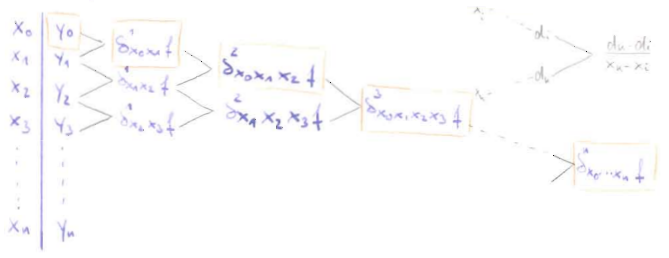
\includegraphics[scale=0.9]{2-interp-aitken.png}
\end{figure}

On admet le résultat que $P_n(X_i) = Y_i$ (démonstration par récurrence avec les formules de Newton).


Formule de Newton : identité algébrique pour toute fonction f
\begin{equation}
    f(X) = TODO
\end{equation}

% exemple


\subsection* {Résolution}

\begin{itemize}
\item Coût du tableau d'Aitken en $O(n^2)$ :

$n + (n - 1) + \cdots + 2 + 1 = \sum_{i = 0}^n i = \frac{n (n + 1)}{2}$
\item $O(n)$ : évaluation du polynôme
\end{itemize}

\bigbreak
Cette méthode se prête à l'ajout de valeurs $(X_i, Y_i)$ à interpoler : il suffit de calculer autant de termes supplémentaires, alors qu'avec Vandermonde et Lagrange il faut tout recalculer.

\bigbreak
$\Rightarrow$ Donc la méthode de Newton est préférable à Vandermonde et Lagrange.

% Graphique


\section {Estimation de l'erreur}

Soit $f \in C^{n + 1}([a,b])$.

$\forall X \in [a,b], \xi \in [a,b]$, on a :

\begin{equation}
\varepsilon(X) = f(X) - P_n(X) = \frac{f^{n + 1}(\xi)}{(n + 1)!} \prod_{i = 0}^n (X - X_i)
\end{equation}


\section {Problème de convergence}

\begin{equation}
\varepsilon_n = f(X) - P_n(X)
\end{equation}


$\varepsilon_n$ ne tend pas vers 0 quand n tend vers l'infini.

En effet, pour toute suite de $X_i$ on peut toujours construire une fonction continue pour laquelle l'interpolation polynomiale ne converge pas.


\section {Phénomène de Runge}

Il existe des fonctions qui montrent ce phénomène de convergence, exemple connu :
\begin{equation}
f(X) = \frac{1}{1 + X^2} \in [-5,5], f \in C^{\infty}
\end{equation}

% Graphique P4

% Graphique P14


\section* {Interpolation polynomiale}

\begin{itemize}
\item Adapté à un petit nombre n de valeurs à interpoler
\item Peu adapté aux données bruitées
\end{itemize}

On observe des problèmes d'oscillation sinon.

On peut diminuer ces problèmes avec un autre choix des abscisses $X_i$ (pas équidistantes), les abscisses de Tchebychev.


\subsection* {Autre solution}

Interpolation par splines (par morceaux) de base avec différents degrés (ex : 3, 5).

% Graphique n = 3


